\section{Validation}
\label{sec:validation}

The model is validated against two published unified models of the near-electrode layers of atmospheric-pressure argon arcs: the near-cathode layer computed by Almeida et al.\ \cite{Almeida2008} and the near-anode layer computed by Semenov et al.\ \cite{semenov2016numerical}. Both works solve the multi-fluid equations for electrons, ions and atoms, with separate electron and heavy-particle temperatures, coupled to Poisson's equation. The two models differ, however, in geometry. Semenov et al.\ use a planar one-dimensional model, as the present one does, so the current density is the same at every \(x\). Almeida et al.\ instead solve their equations in spherical symmetry about a hemispherical cathode of radius \(r_c=1\)~mm, so their current density decreases with distance as \(j_c\,r_c^2/(r_c+x)^2\), whereas the present model keeps \(j=j_c\) throughout. At the outer boundary of their domains, which is 1~cm from the electrode, both assume that the plasma is uniform and in LTE, with Joule heating balanced by radiation alone. Their solutions show, however, that the plasma is already close to LTE much nearer the electrode: at \(x=5\times10^{-4}\)~m, \(T_e\) and \(T_h\) differ by less than 0.3\,\% in both published solutions, and the charged-particle density is within 2\,\% of the Saha density, although the plasma there is not yet uniform. We therefore restrict the present domain to this length and take the boundary condition at \(x=L\) from the published solutions.

The conditions of the published calculations were reproduced as closely as possible. The electrode surface temperature was prescribed at the value used by Almeida et al.\ and Semenov et al., respectively, rather than obtained from the heat balance~(\ref{eq:bc-heat-balance}), and the radial loss~(\ref{eq:radial-loss}) was switched off, \(\Lambda=0\), since neither model includes it. The domain was discretized as described in Section~\ref{sec:numerics}. Throughout the space-charge sheath, the region where \(|n_i-n_e|/n_i>1\,\%\) (\(x\lesssim1.1\ \mu\)m at the cathode and \(0.7\ \mu\)m at the anode), the cells are smaller than the local electron Debye length, by a factor of at least 1.5 at the cathode and 6 at the anode. The equations were integrated in time at a fixed current density to a steady state. 

\begin{figure}[t]
\centering
\begin{minipage}[t]{0.485\textwidth}
\centering
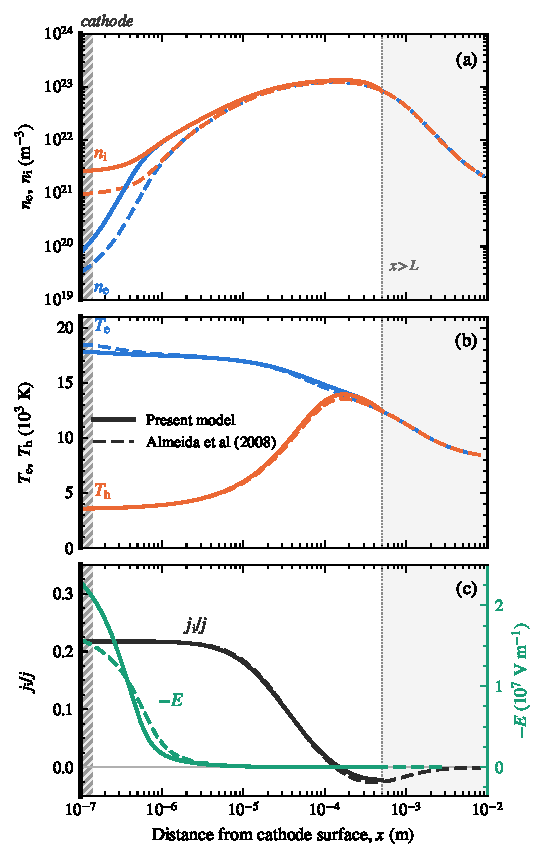
\includegraphics[height=10.5cm]{figures/validation_fig/almeida_J1e7/compareJ1e7_plt00800.pdf}
\caption{Near-cathode layer in argon at atmospheric pressure, cathode surface temperature \(T_{\rm w}=3500\)~K and current density \(j_c=10^7\ \mathrm{A\,m^{-2}}\): present model (solid lines) and Almeida et al.\ \cite{Almeida2008} (dashed lines, figures~5(b) and 6). (a) Electron and ion number densities. (b) Electron and heavy-particle temperatures. (c) Ion fraction of the current density, \(j_i/j\) (left axis), and field strength \(-E\) (right axis). The hatched strip at the left marks the cathode surface. The shaded region, \(x>L\), lies outside the computational domain.}
\label{fig:val-cathode}
\end{minipage}\hfill
\begin{minipage}[t]{0.485\textwidth}
\centering
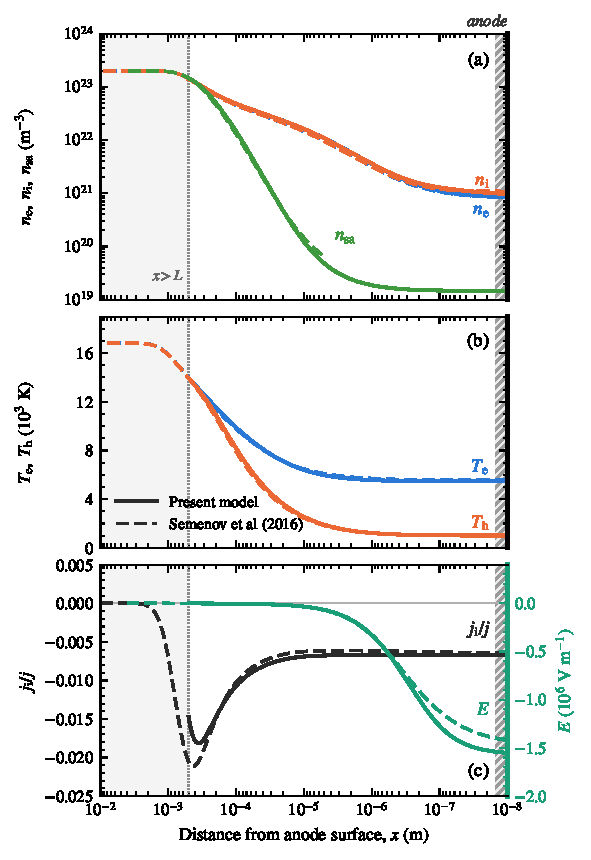
\includegraphics[height=10.5cm]{figures/validation_fig/semenov_J1.5e7/compareJ1.5e7_plt00340.pdf}
\caption{Near-anode layer in argon at atmospheric pressure, anode surface temperature \(T_{\rm s}=1000\)~K and current density \(j=1.5\times10^7\ \mathrm{A\,m^{-2}}\): present model (solid lines) and Semenov et al.\ \cite{semenov2016numerical} (dashed lines, figures~3(b), 4 and 5). (a) Electron and ion number densities and the Saha density \(n_{\rm sa}\). (b) Electron and heavy-particle temperatures. (c) Ion fraction of the current density, \(j_i/j\) (left axis), and electric field \(E\) (right axis). The distance axis is reversed, so that the anode surface, marked by the hatched strip, is at the right. The shaded region, \(x>L\), lies outside the computational domain.}
\label{fig:val-anode}
\end{minipage}
\end{figure}

\subsection{Near-cathode layer}
\label{sec:val-cathode}
Almeida et al.\ \cite{Almeida2008} computed the near-cathode layer of an atmospheric-pressure argon arc for three current densities, and concluded that only one of these cases is realizable in practice: a tungsten cathode with a work function of \(4.55\)~eV, thermionic emission~(\ref{eq:bc-emission}) included, a surface temperature of \(3500\)~K and a current density of \(10^7\ \mathrm{A\,m^{-2}}\). We therefore model this case; the two solutions are compared in figure~\ref{fig:val-cathode}. The temperature profiles agree closely across the whole layer (figure~\ref{fig:val-cathode}(b)). The electron temperature stays near \(17.5\)--\(18\)~kK through the sheath and the inner part of the ionization layer and decreases towards the bulk plasma, while the heavy-particle temperature rises from the wall value to a maximum of \(13.9\)~kK at \(x\approx2\times10^{-4}\)~m, compared with \(13.6\)~kK in the solution of Almeida et al. From \(x\approx3\times10^{-6}\)~m outwards, both temperatures agree with theirs within \(0.4\)~kK (3\,\%).

The ion fraction of the current, figure~\ref{fig:val-cathode}(c), is reproduced over the whole layer. At the cathode surface the present model gives \(j_i/j=0.218\), compared with \(0.216\) reported by Almeida et al.; \(j_i/j\) stays at this value through the sheath, falls to zero at \(x\approx1.5\times10^{-4}\)~m, and becomes slightly negative further out, where the ion flux is directed away from the cathode. Almeida et al.\ also place the sheath edge where the charge separation reaches 1\,\%. The present model gives a sheath voltage of \(9.96\)~V at \(x_{\rm s}=1.1\ \mu\)m, compared with \(10.2\)~V at \(x_{\rm s}=1.5\ \mu\)m in their solution. In the ionization layer, \(10^{-5}\lesssim x\lesssim3\times10^{-4}\)~m, the charged-particle densities of the present model are 7--15\,\% higher than theirs (figure~\ref{fig:val-cathode}(a)). The largest differences are in the space-charge sheath, \(x\lesssim10^{-6}\)~m. At \(x=10^{-7}\)~m, the electron and ion densities of the present model are higher by a factor of about 2.5, and the field strength is \(2.3\times10^7\ \mathrm{V\,m^{-1}}\), compared with \(1.6\times10^7\ \mathrm{V\,m^{-1}}\).



\subsection{Near-anode layer}
\label{sec:val-anode}

The anode case is that of figure~3(b) of Semenov et al.\ \cite{semenov2016numerical}: a non-emitting anode, \(\Gamma_{\rm em}=0\), with surface temperature \(1000\)~K and current density \(1.5\times10^7\ \mathrm{A\,m^{-2}}\). The comparison is shown in figure~\ref{fig:val-anode}. The electron and ion densities agree with those of Semenov et al.\ within 15\,\% across the layer (figure~\ref{fig:val-anode}(a)). Following Semenov et al., the figure also shows the Saha density \(n_{\rm sa}\), the charged-particle density that the local \(T_e\) and \(T_h\) would give in ionization equilibrium with quasi-neutrality at the pressure \(p_0\). Near the anode the actual densities exceed \(n_{\rm sa}\) by nearly two orders of magnitude. The anode region is therefore far from ionization equilibrium: charged particles are supplied by diffusion from the hotter plasma rather than produced locally, and both models capture this departure.

The temperature profiles agree closely (figure~\ref{fig:val-anode}(b)). At the anode surface, the electron temperature is \(5.46\)~kK, compared with \(5.59\)~kK reported by Semenov et al., and the heavy-particle temperatures differ by less than \(0.3\)~kK across the layer. The electric field near the anode, figure~\ref{fig:val-anode}(c), is negative: it is directed towards the anode, so that the anode lies at a lower potential than the adjacent plasma and the electrons are retarded. The field at the surface is \(-1.57\times10^6\ \mathrm{V\,m^{-1}}\), compared with \(-1.42\times10^6\ \mathrm{V\,m^{-1}}\) in the solution of Semenov et al. Ions flow into the anode, so \(j_i/j\) is negative there. At the surface, the present model gives \(j_i/j=-0.0067\), compared with their \(-0.0065\). With the same definition of the sheath edge as at the cathode, the present model gives \(x_{\rm s}=0.70\ \mu\)m and \(\phi_{\rm s}=0.58\)~V, compared with \(0.71\ \mu\)m and \(0.54\)~V obtained from the density and field profiles of Semenov et al.

The main difference is in the minimum of \(j_i/j\), which is \(-0.018\) at \(x=3.5\times10^{-4}\)~m in the present model and \(-0.021\) at \(x=4.3\times10^{-4}\)~m in the solution of Semenov et al. This difference reflects the different models. Imposing their state at \(x=L\) fixes the values of the densities and temperatures there, but not their gradients, which follow from each model's governing equations, and \(j_i/j\) depends on these gradients. 

The present model reproduces the structure of the near-electrode layer for both cathode and anode cases: the temperatures, the current partition between ions and electrons, the sign and magnitude of the near-electrode field, the sheath voltages (within 2.5\,\% at the cathode and 7\,\% at the anode) and the departure from ionization equilibrium. Apart from the charged-particle densities in the cathode sheath and the minimum of \(j_i/j\) near the outer boundary of the anode calculation, the temperatures agree within 3--5\,\% and the charged-particle densities within 15\,\%. The differences most likely arise from the different descriptions of the transport properties (Appendix~\ref{app:transport}) and of the ion boundary condition~(\ref{eq:bc-ion}).
